\section{ARDUINO}

Una buena definición de lo que es Arduino lo da la Wikipedia; <<Arduino es una plataforma de hardware libre, basada en una placa con un microcontrolador y un entorno de desarrollo, diseñada para facilitar el uso de la electrónica en proyectos multidisciplinares.>>.

Para este proyecto de fin de grado se va a utilizar \emph{Arduino} para desarrollar el hardware que permita la lectura de códigos de barras de los productos. Para ello se va a contar con una placa \emph{Arduino Yún} y distintos componentes como una pantalla TFT, un lector de código de barras y diversos componentes como resistencias y pulsadores.

A continuación se va a explicar brevemente el hardware \emph{Arduino}, \emph{Arduino Yún} y una pantalla TFT desarrollada para \emph{Arduino}.

\subsection{Hardware}

El hardware consiste en una placa con un microcontrolador \emph{Atmel AVR} y puertos de entrada/salida. Los microcontroladores más usados son el \emph{Atmega168}, \emph{Atmega328}, \emph{Atmega1280}, \emph{ATmega8} por su sencillez y bajo coste que permiten el desarrollo de múltiples diseños.

\begin{figure}[h!]
    \centering
    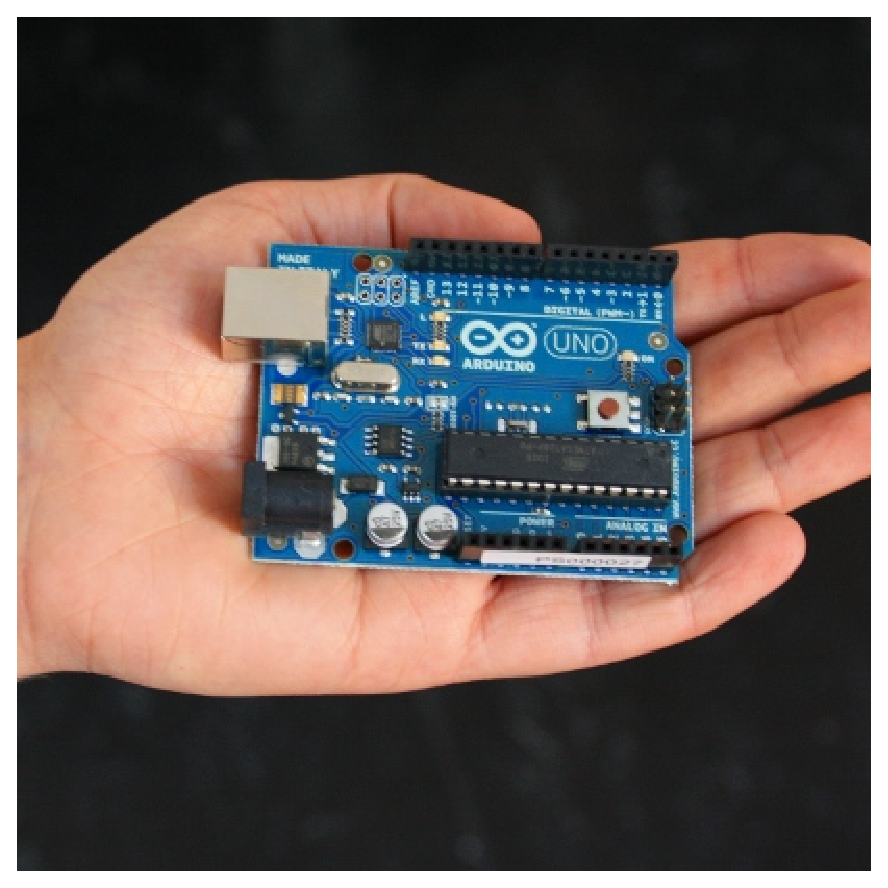
\includegraphics[keepaspectratio,width=0.6\textwidth]{arduino_uno_test.eps}
    \caption{Arduino uno}\label{fig:arduino_uno_test}
\end{figure}


Por otro lado el software consiste en un entorno de desarrollo que implementa el lenguaje de programación \emph{Wiring} y el cargador de arranque que es ejecutado en la placa.

\begin{figure}[h!]
    \centering
    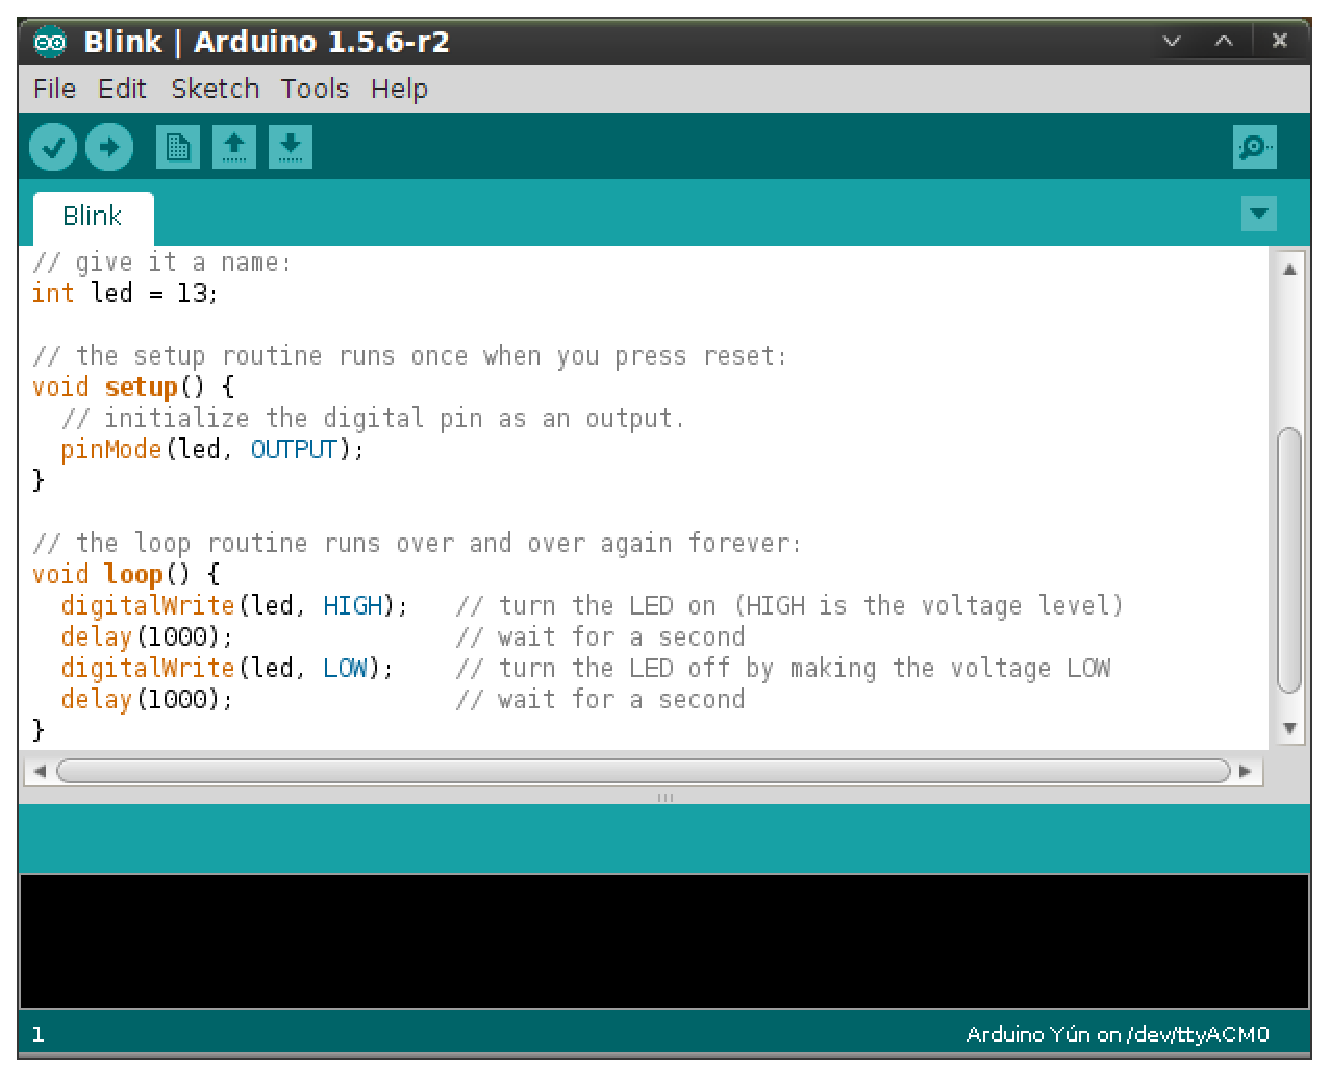
\includegraphics[keepaspectratio,width=0.6\textwidth]{arduino-ide.eps}
    \caption{IDE Arduino}\label{fig:arduino-ide}
\end{figure}

El lenguaje de alto nivel \emph{Wiring}, implementado en C/C++, permite una programación sencilla del hardware. Comparte todas las funciones estándar de C, algunas de C++ y añade las propias para el manejo de puertos (digitales, analógicos).

A continuación se muestra un código sencillo para hacer parpadear un diodo led cada segundo, se utiliza el puerto 8 digital de la placa \emph{Arduino}:

\begin{lstlisting}
    void setup() {
      pinMode(8, OUTPUT);
    }

    boolean encendido = false;
    void loop() {
      if(!encendido) {
        digitalWrite(8, HIGH);
      } else {
        digitalWrite(8, LOW);
      }
      encendido!=encendido;
      delay(1000);
    }
\end{lstlisting}

\subsection{Arduino Yún}

Existen una gran variedad de placas Arduino, tanto oficiales como no oficiales; Arduino uno, Arduino Mega, Arduino Leonardo... Y una de las más recientes, la cual usaré en este proyecto, es la placa \emph{Arduino Yún}.

\begin{figure}[h!]
    \centering
    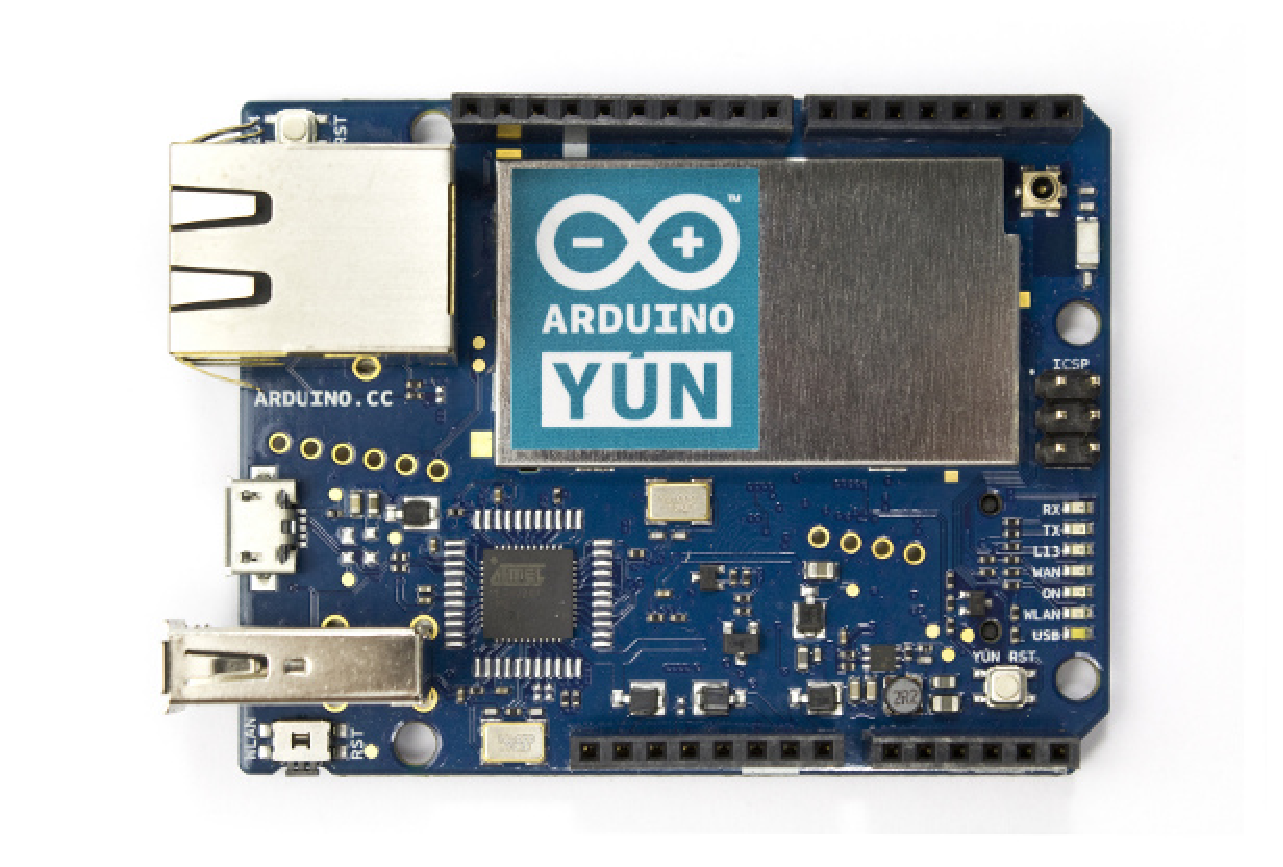
\includegraphics[keepaspectratio,width=0.6\textwidth]{arduino_yun_front.eps}
    \caption{Frontal arduino}\label{fig:arduino-yun-front}
\end{figure}

La ventaja principal, y por la que me he decantado por comprar esta placa, es la combinación de Arduino (\emph{ATmega 32U4}) con un sistema operativo Linux (\emph{AR9331}) con conectividad Wi-Fi. Esto permite utilizar todo el potencial de Arduino en el desarrollo de nuestro hardware y obtener todo el potencial de una máquina Linux, a través del sistema operativo \emph{Linino}, para ejecutar comandos, scripts, aplicaciones y cualquier cosa que se nos ocurra.

\begin{figure}[h!]
    \centering
    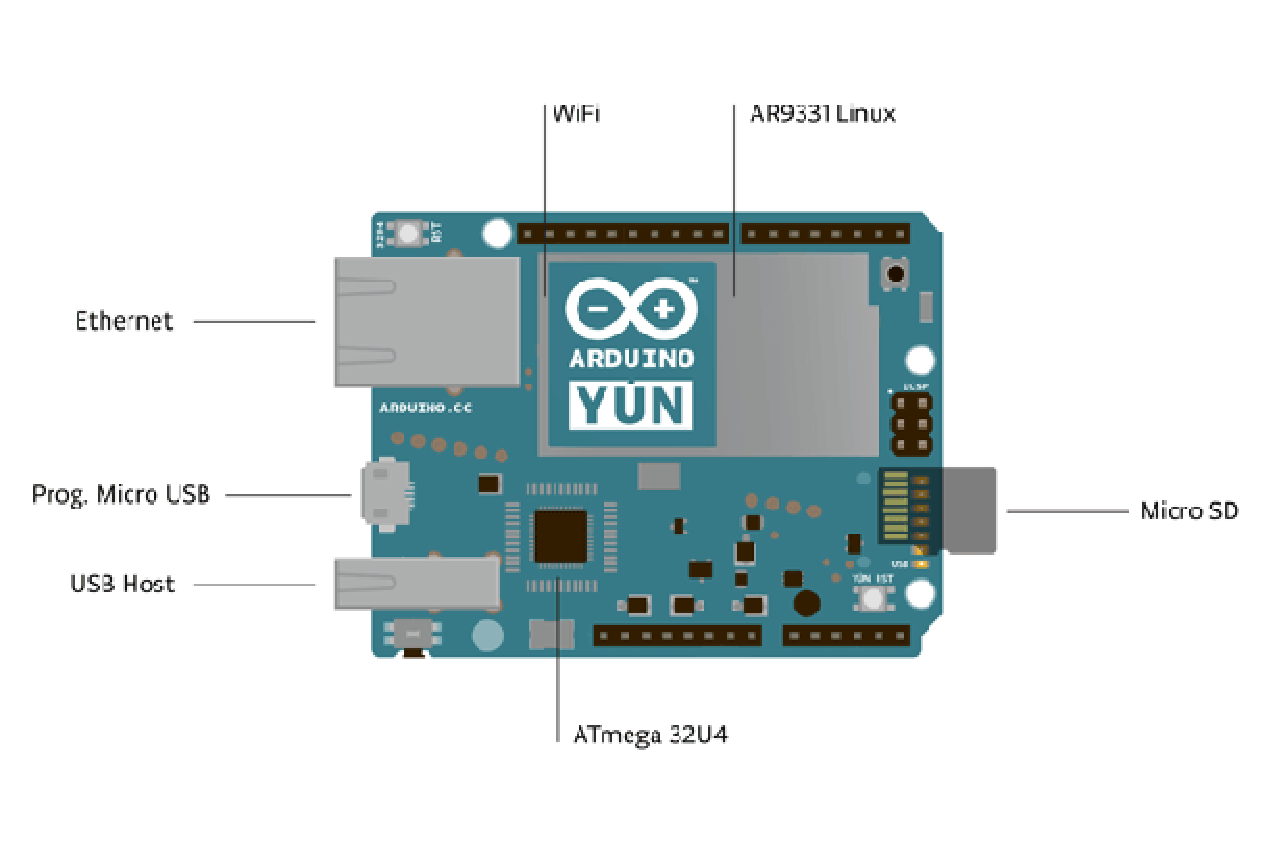
\includegraphics[keepaspectratio,width=0.6\textwidth]{arduino_parts.eps}
    \caption{Componentes de arduino}\label{fig:arduino-parts}
\end{figure}

La comunicación entre Arduino y Linux se realiza a través de la librería \emph{Bridge}, facilitando la comunicación entre los dos procesadores. La librería da la habilidad a Arduino y correr scripts, comunicarse con interfaces de red y recibir información del procesador \emph{AR9331}. El Host USB, las interfaces de red y el lector de tarjetas de memoria están conectados al procesador \emph{AR9331} manejado por Linux, la librería Bridge también permite a Arduino acceder a estos periferios.

Las características de \emph{Arduino Yún} son las siguientes:

\textbf{AVR Arduino microcontroller}

\begin{tabular}{| l | l |}
\hline
Microcontroller & ATmega32u4 \\ \hline
Operating Voltage & 5V \\ \hline
Input Voltage & 5V \\ \hline
Digital I/O Pins & 20 \\ \hline
PWM Channels & 7 \\ \hline
Analog Input Channels & 12 \\ \hline
DC Current per I/O Pin & 40 mA \\ \hline
DC Current for 3.3V Pin & 50 mA \\ \hline
Flash Memory & 32 KB (of which 4 KB used by bootloader) \\ \hline
SRAM & 2.5 KB \\ \hline
EEPROM & 1 KB \\ \hline
Clock Speed & 16 MHz \\ \hline
\end{tabular}

\textbf{Linux microprocessor}

\begin{tabular}{| l | l |}
\hline
Processor & Atheros AR9331 \\ \hline
Architecture & MIPS @400MHz \\ \hline
Operating Voltage & 3.3V \\ \hline
Ethernet & IEEE 802.3 10/100Mbit/s \\ \hline
WiFi & IEEE 802.11b/g/n \\ \hline
USB Type-A & 2.0 Host/Device \\ \hline
Card Reader & Micro-SD only \\ \hline
RAM & 64 MB DDR2 \\ \hline
Flash Memory & 16 MB \\ \hline
\end{tabular}


\subsection{Pantalla TFT}

Uno de los componentes para dotar de comunicación a nuestra placa Arduino es utilizar una pantalla TFT. Existen variedad de pantallas TFT; diferentes dimensiones, con soporte táctil, mayor rapidez de refresco... Para el proyecto he optado por comprar la oficial de Arduino:

\begin{figure}[h!]
    \centering
    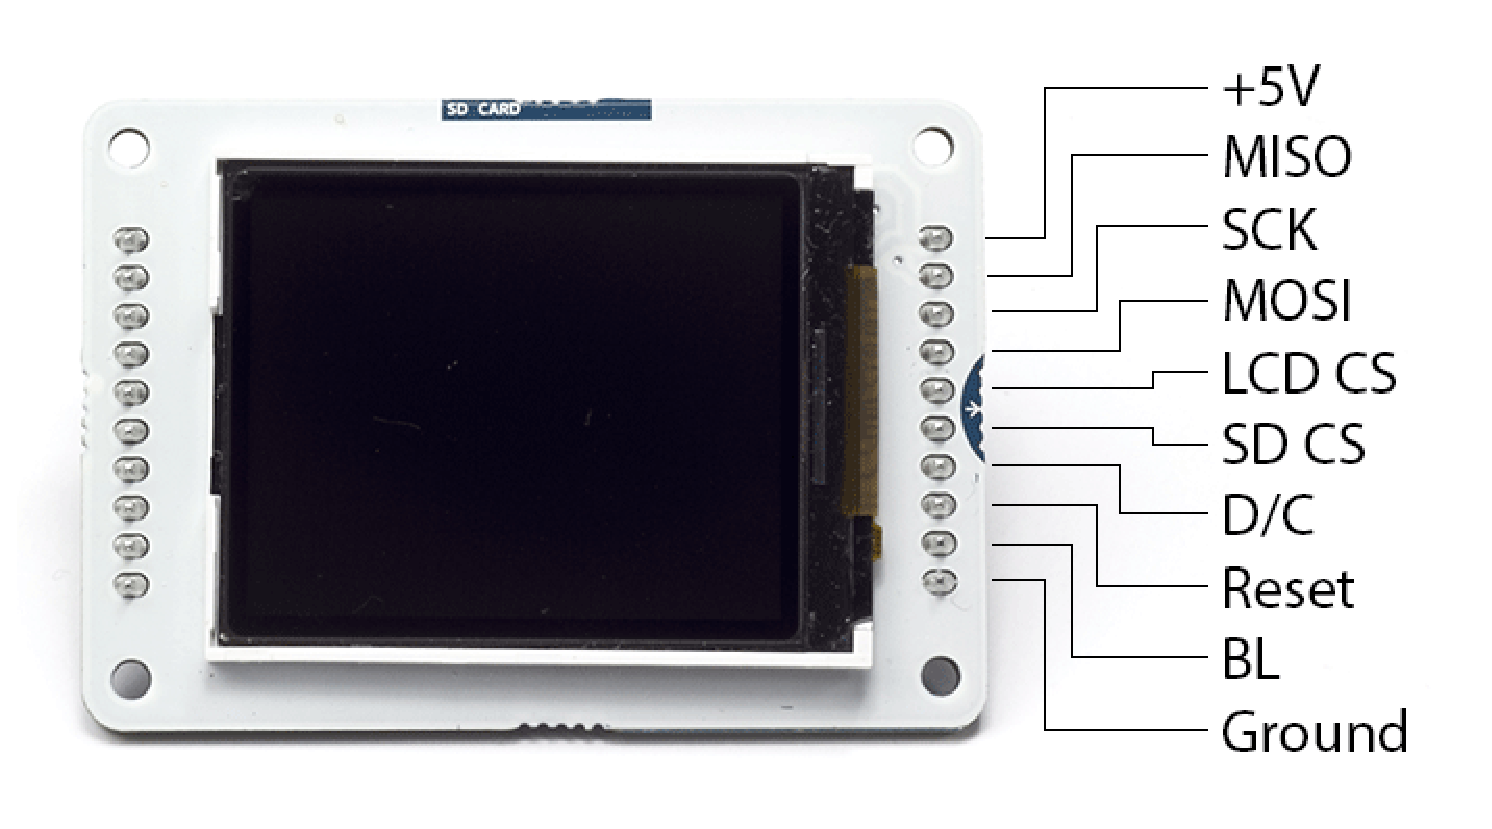
\includegraphics[keepaspectratio,width=0.6\textwidth]{pantalla_tft_front.eps}
    \caption{Pantalla TFT}\label{fig:arduino-tft-front}
\end{figure}


\parpic[r][]{
    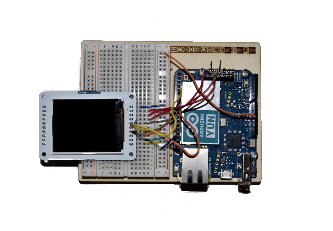
\includegraphics[keepaspectratio,width=0.38\textwidth]{arduino_conexiones.eps}
    \label{fig:arduino_conexiones}
}

Es una pantalla de 1,77" de diagonal, con 160x128 pixels de resolución, y con un lector de tarjetas SD para cargar imágenes. La pantalla está pensada para encajar con las placas \emph{Arduino Esplora} ó \emph{Arduino Robot}, con el resto de placas Arduino se pueden realizar las conexiones a mano.

A través de la librería \emph{TFT} podemos dibujar elementos en la pantalla o, mediante una memoria SD, cargar imagenes desde la tarjeta en la pantalla. A continuación expongo una manera para dibujar un círculo y un cuadrado en la pantalla:

\begin{lstlisting}
    ...

    void setup() {
      TFTscreen.begin();
      TFTscreen.background(255, 255, 255);

    }

    void loop() {
      TFTscreen.stroke(0,0,0);
      TFTscreen.fill(127,127,127);
      TFTscreen.circle(TFTscreen.width()/2, TFTscreen.height()/2, 30);

      TFTscreen.fill(50,40,30);
      TFTscreen.rect(TFTscreen.width()/2, TFTscreen.height()/2, 30, 30);

      delay(1500);
    }
\end{lstlisting}

A continuación se muestra una captura de como se visualiza el dibujo en la pantalla:

\begin{figure}[h!]
    \centering
    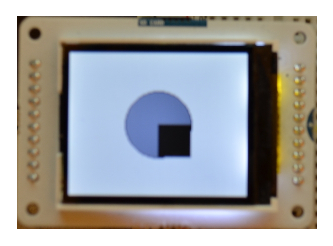
\includegraphics[keepaspectratio,width=0.4\textwidth]{tft_circulo_cuadrado.eps}
    \caption{TFT - Dibujando}\label{fig:tft_circulo_cuadrado}
\end{figure}

En cambio, para cargar una imagen desde la tarjeta de memoria y mostrarla en la pantalla TFT, primero tenemos que esperar a que la memoria SD esté inicializada y a continuación, leer la imagen y renderizarla en pantalla:

\begin{lstlisting}
    ...

    void setup() {
      TFTscreen.begin();
      TFTscreen.background(255, 255, 255);

      if (!SD.begin(sd_cs)) {
        return; // Error SD
      }
    }

    void loop() {
      logo = TFTscreen.loadImage("f1.bmp");
      TFTscreen.image(logo, 0, 0);
      delay(1500);
    }
\end{lstlisting}

A continuación se muestra una captura de como se visualiza la imagen en la pantalla:

\begin{figure}[h!]
    \centering
    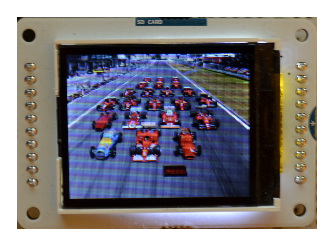
\includegraphics[keepaspectratio,width=0.4\textwidth]{tft_f1.eps}
    \caption{TFT - Imagen}\label{fig:tft_f1}
\end{figure}

\subsection{RFID}

\parpic[r][]{
    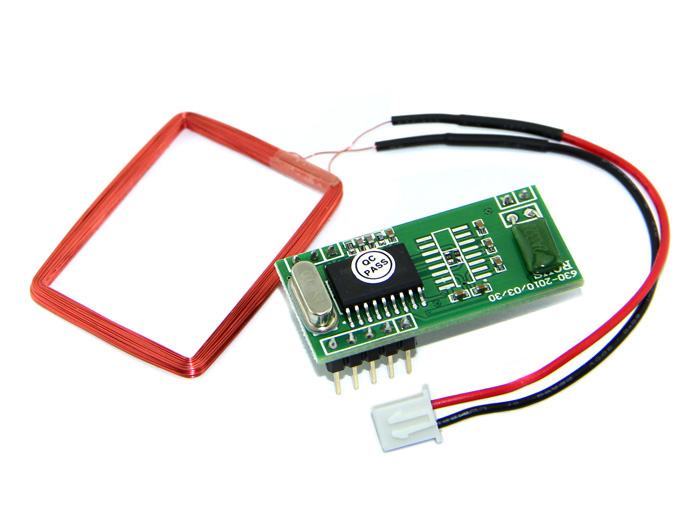
\includegraphics[keepaspectratio,width=0.38\textwidth]{lector_rfid.png}
    \label{fig:lector_rfid}
}

El lector \emph{RFID} es uno de los componentes empleados para poder escanear productos. En concreto se ha utilizado para el proyecto un lector \emph{RFID de 125K} con las siguientes características:

\begin{itemize}
    \item Working voltage: 3.5-5V
    \item Frequency: 125Khz
    \item Baud rate: 9600
    \item Interface Type: TTL Level RS232 format
    \item Reception range: 30mm~50mm
\end{itemize}

El código para trabajar con el lector \emph{RFID} es muy sencillo, la única ''complicación'' es tener que utilizar la librería \emph{SoftwareSerial} para simular dos pintes como puerto serie.

No se pueden utilizar los pines dedicados de puerto serie (\emph{0 y 1}) ya que \emph{Arduino Yún} los utiliza para la comunicación entre el microcontrolador \emph{ATmega32U4} y el microprocesador \emph{Atheros AR9331} a través de la librería \emph{Bridge}.

El código utilizado para escanear tarjetas \emph{RFID} es el siguiente:

\begin{lstlisting}
//Lector RFID
#include <SoftwareSerial.h>
#define rxPin 11
#define txPin 12
SoftwareSerial RFID = SoftwareSerial(rxPin, txPin); // RX and TX
char arrayTag[10];

void setup() {
    RFID.begin(9600);
}

void loop() {
    if(leerYProcesarEtiquetaRFID()) {
        // Hacer algo
    }
}

boolean leerYProcesarEtiquetaRFID() {
  int leidoTag = 0;

  String tag;
  while(RFID.available() > 0) {
      leidoTag = 1;
      int rfid = RFID.read();

      if(rfid != 13 && rfid != 10) {
         tag += (char)rfid;
      }
  }
  if(leidoTag) {
    tag.toCharArray(arrayTag, 10);
  }

  return leidoTag != 0;
}
\end{lstlisting}

